\documentclass[a4paper, 12pt]{article}
\usepackage[top=1.8cm, bottom=1.8cm, left=1.5cm, right=1.5cm]{geometry}
\usepackage{float}
\usepackage[utf8]{inputenc}
\usepackage{pgfplots}
\pgfplotsset{width=10cm, compat=1.18}


\begin{document}
	
	\begin{center}
		Universidade Federal do Rio Grande do Norte
		
		Departamento de Engenharia da Computação e Automação  
		
		DCA3703 - Programação Paralela  
		
		\textbf{Tarefa 16: Comunicação Coletiva com MPI}  
		
		\textbf{Aluno:} Daniel Bruno Trindade da Silva  
	\end{center}  
	
	\section{Introdução}
	
	\hspace{0.62cm}Este relatório tem como objetivo apresentar os conhecimentos adquiridos durante a realização da Tarefa 16 da disciplina de \textbf{Programação Paralela}. A atividade teve como objetivo mensurar o tempo de comunicação entre os processos usando ferramentas do MPI. Para isso será realizada a implementação e análise de um programa que simule a difusão de calor em uma barra 1D. 
	
	\section{Enunciado}
	
	\hspace{0.62cm}Implemente um programa MPI que calcule o produto $y = A \cdot x$, onde A é uma matriz M×N e x é um vetor de tamanho N. Divida a matriz A por linhas entre os processos com \texttt{MPI\_Scatter}, e distribua o vetor x inteiro com \texttt{MPI\_Bcast}. Cada processo deve calcular os elementos de y correspondentes às suas linhas e enviá-los de volta ao processo 0 com \texttt{MPI\_Gather}. Compare os tempos com diferentes tamanhos de matriz e número de processos.
	
	\section{Desenvolvimento}
	\hspace{0.62cm}O código desenvolvido tem como objetivo realizar o produto matriz-vetor de forma paralela utilizando a biblioteca MPI (Message Passing Interface). Para otimizar o uso de memória, optamos por utilizar o tipo de dado \texttt{uint8\_t} (inteiro sem sinal de 8 bits), uma vez que os elementos da matriz e do vetor são pequenos, e o uso desse tipo reduz significativamente o consumo de memória. Essa escolha foi especialmente importante devido ao tamanho expressivo das matrizes processadas, que podem chegar a 32768 x 32768 elementos, representando mais de 2 GB de dados se fossem utilizados tipos de maior tamanho, como int ou double.
	
	\subsection{Comunicação entre Processos com MPI}
	\hspace{0.62cm}Na implementação, utilizamos três operações fundamentais de comunicação da biblioteca MPI:
	\begin{itemize}
		\item \textbf{\texttt{MPI\_Bcast}}: Esta função foi utilizada para realizar o broadcast do vetor x para todos os processos. Como o vetor x é necessário para o cálculo local de cada processo, foi essencial garantir que todos os processos tivessem acesso à mesma cópia deste vetor. O processo com rank 0 inicializa o vetor e, em seguida, o \texttt{MPI\_Bcast} propaga os dados a todos os demais processos de forma eficiente.
		
		\item \textbf{\texttt{MPI\_Scatter}}: Utilizamos esta função para distribuir as partes da matriz A entre os processos. Como cada processo é responsável pelo cálculo de uma parte do vetor resultado y, foi necessário dividir as linhas da matriz A igualmente entre eles. O \texttt{MPI\_Scatter} possibilitou essa divisão automática e eficiente, enviando a cada processo apenas os dados necessários para o seu cálculo.
		
		\item \textbf{\texttt{MPI\_Gather}}: Após o cálculo paralelo, cada processo obteve uma parte do vetor y. Utilizamos o \texttt{MPI\_Gather} para coletar essas partes e reunir o vetor resultado completo no processo com rank 0, que então pode realizar o processamento final ou análise dos dados.
	\end{itemize}
	
	Além disso, para avaliar o desempenho, foi desenvolvido um script automatizado que permite executar o programa variando tanto o tamanho da matriz quanto o número de processos utilizados. Esse script facilitou a realização de diversos experimentos, possibilitando a coleta de dados para analisar o comportamento do código em diferentes cenários de execução, como o impacto da divisão de trabalho entre processos e a eficiência do paralelismo.
	
	\section{Resultados}
		\begin{table}[h!]
		\centering
		\label{tab:execution_times_simple}
		\begin{tabular}{|l|c|c|c|c|c|}
			\hline
			\textbf{Tamanho da Matriz} & \multicolumn{5}{c|}{\textbf{Número de Processos}} \\
			\cline{2-6}
			& \textbf{2} & \textbf{4} & \textbf{8} & \textbf{16} & \textbf{32} \\
			\hline
			$2048 \times 2048$        & 0.007393   & 0.012269   & 0.010754   & 0.017535    & 0.032846    \\ % source 1, 2
			\hline
			$4096 \times 4096$        & 0.024350   & 0.019467   & 0.026092   & 0.018572    & 0.033169    \\ % source 3, 4
			\hline
			$8192 \times 8192$        & 0.223196   & 0.174600   & 0.149724   & 0.073371    & 0.080450    \\ % source 5
			\hline
			$16384 \times 16384$      & 0.336517   & 0.201913   & 0.159433   & 0.076215    & 0.075465    \\ % source 6, 7
			\hline
			$32768 \times 32768$      & 1.314407   & 0.773659   & 0.510369   & 0.249389    & 0.193285    \\ % source 8
			\hline
		\end{tabular}
		\caption{Tempo de Execução (s) por Tamanho da Matriz e Número de Processos}
	\end{table}
	
	
	\begin{figure}[h!]
		\centering
		\begin{tikzpicture}
			\begin{axis}[
				title={Performance de Processamento de Matrizes},
				xlabel={Tamanho da Matriz ($N \times N$)},
				ylabel={Tempo de Execução (s)},
				xmode=log, % Using log scale for matrix size due to large differences
				ymode=log, % Using log scale for time as well, common for performance plots
				legend pos=north west, % Position the legend
				grid=major, % Add a grid
				width=0.9\textwidth, % Adjust width
				height=0.4\textheight, % Adjust height
				xtick={2048, 4096, 8192, 16384, 32768}, % Specify x-axis ticks
				xticklabels={$2048$, $4096$, $8192$, $16384$, $32768$},
				xticklabel style={anchor=center, yshift=-10pt}, % Rotate x-axis labels for better readability
				log basis x=2, % Base for log scale on x-axis
				log basis y=10, % Base for log scale on y-axis
				]
				
				% Data for 2 processos
				\addplot+ [mark=*, line width=1.2pt] coordinates {
					(2048, 0.007393) % Source 1
					(4096, 0.024350) % Source 3
					(8192, 0.223196) % Source 5
					(16384, 0.336517) % Source 6
					(32768, 1.314407) % Source 8
				};
				\addlegendentry{2 Processos}
				
				% Data for 4 processos
				\addplot+ [mark=square*, line width=1.2pt] coordinates {
					(2048, 0.012269) % Source 2
					(4096, 0.019467) % Source 3
					(8192, 0.174600) % Source 5
					(16384, 0.201913) % Source 6
					(32768, 0.773659) % Source 8
				};
				\addlegendentry{4 Processos}
				
				% Data for 8 processos
				\addplot+ [mark=triangle*, line width=1.2pt] coordinates {
					(2048, 0.010754) % Source 1
					(4096, 0.026092) % Source 3
					(8192, 0.149724) % Source 5
					(16384, 0.159433) % Source 6
					(32768, 0.510369) % Source 8
				};
				\addlegendentry{8 Processos}
				
				% Data for 16 processos
				\addplot+ [mark=diamond*, line width=1.2pt] coordinates {
					(2048, 0.017535) % Source 1
					(4096, 0.018572) % Source 3
					(8192, 0.073371) % Source 5
					(16384, 0.076215) % Source 6
					(32768, 0.249389) % Source 8
				};
				\addlegendentry{16 Processos}
				
				% Data for 32 processos
				\addplot+ [mark=pentagon*, line width=1.2pt] coordinates {
					(2048, 0.032846) % Source 1
					(4096, 0.033169) % Source 4
					(8192, 0.080450) % Source 5
					(16384, 0.075465) % Source 7
					(32768, 0.193285) % Source 8
				};
				\addlegendentry{32 Processos}
				
			\end{axis}
		\end{tikzpicture}
		\caption{Gráfico de Linhas do Tempo de Execução pelo Tamanho da Matriz para Diferentes Números de Processos.}
		\label{fig:matrix_performance}
	\end{figure}
	
	\section{Analise dos Resultados}
	
	\subsection{Ganhos de Desempenho}
	\hspace{0.62cm}Observa-se que, conforme o número de processos aumenta, o tempo de execução tende a diminuir, principalmente para matrizes de maior dimensão. Por exemplo, para a matriz de 32.768 x 32.768, o tempo de execução reduziu de 1,31 segundos com 2 processos para apenas 0,19 segundos com 32 processos. Esse resultado evidencia a eficiência do paralelismo e a capacidade de dividir a carga computacional entre múltiplos processos, reduzindo significativamente o tempo total de execução.
	
	Esse comportamento é característico de algoritmos que possuem grande potencial de paralelização, como o produto matriz-vetor, onde o trabalho pode ser dividido de forma relativamente equilibrada entre os processos. A função \texttt{MPI\_Scatter} foi fundamental para distribuir de forma eficiente as linhas da matriz, enquanto o uso de \texttt{MPI\_Bcast} garantiu que todos os processos tivessem acesso ao vetor x com um custo de comunicação relativamente baixo.
	
	\subsection{Efeito do Overhead de Comunicação}
	\hspace{0.62cm}No entanto, para matrizes menores, como a de 2.048 x 2.048, o aumento do número de processos nem sempre resulta em uma melhora significativa no tempo de execução. Por exemplo, o tempo com 2 processos foi de 0,0073 segundos, enquanto com 32 processos foi de 0,0328 segundos, representando uma piora no desempenho.
	
	Esse comportamento é explicado pelo overhead de comunicação: quando a quantidade de dados processados por cada processo é muito pequena, o custo das operações de comunicação (\texttt{MPI\_Scatter}, \texttt{MPI\_Bcast} e \texttt{MPI\_Gather}) acaba sendo mais relevante do que o tempo gasto efetivamente no cálculo. Assim, para matrizes pequenas, o uso de um número elevado de processos não compensa, podendo inclusive degradar a performance.
	
	\vspace{.5cm}
	
	Em síntese, os resultados obtidos demonstram que:
	
	\begin{itemize}
		\item O paralelismo com MPI proporciona ganhos de desempenho significativos para o produto matriz-vetor, principalmente com matrizes de grande dimensão.
		
		\item Existe um ponto de equilíbrio entre o número de processos e o tamanho da matriz, sendo que, para matrizes pequenas, o excesso de processos pode aumentar o tempo de execução devido ao overhead de comunicação.
	\end{itemize}
	
	\section{Conclusão}
	
	\hspace{0.62cm}A realização desta atividade permitiu consolidar conhecimentos importantes sobre a programação paralela utilizando a biblioteca MPI, com foco no uso de operações de comunicação coletiva como \texttt{MPI\_Bcast}, \texttt{MPI\_Scatter} e \texttt{MPI\_Gather}. A implementação do produto matriz-vetor demonstrou na prática como a divisão de tarefas entre múltiplos processos pode acelerar significativamente a execução de operações computacionalmente intensivas.
	
	Os experimentos realizados evidenciaram que o paralelismo é altamente eficaz para problemas de grande dimensão, proporcionando uma redução expressiva no tempo de execução à medida que o número de processos aumenta. Por outro lado, observou-se que para problemas menores, o \textit{overhead} associado à comunicação entre processos pode superar os ganhos obtidos pela divisão do trabalho, o que reforça a importância de avaliar cuidadosamente o balanceamento entre carga computacional e custo de comunicação em aplicações paralelas.
	
	Por fim, esta tarefa reforçou a importância do paralelismo na solução de problemas de larga escala e destacou o papel crucial das técnicas de comunicação coletiva para o desenvolvimento de aplicações eficientes e escaláveis.
	
\end{document}
